\documentclass[12pt]{article}
 \usepackage[margin=1in]{geometry} 
\usepackage{amsmath,amsthm,amssymb,amsfonts, enumitem, fancyhdr, color, comment, graphicx, environ}
\pagestyle{fancy}
\setlength{\headheight}{65pt}
\newenvironment{problem}[2][Problem]{\begin{trivlist}
\item[\hskip \labelsep {\bfseries #1}\hskip \labelsep {\bfseries #2.}]}{\end{trivlist}}
\newenvironment{sol}
    {\emph{Solution:}
    }
    {
    \qed
    }
\specialcomment{com}{ \color{blue} \textbf{Comment:} }{\color{black}}
\NewEnviron{probscore}{\marginpar{ \color{blue} \tiny Problem Score: \BODY \color{black} }}
\usepackage[UTF8]{ctex}
\lhead{Name: 陈稼霖\\ StudentID: 45875852}
\rhead{PHYS1304 \\ Electrodynamics \\ Spring 2019 \\ Homework 3}
\begin{document}
\begin{problem}{1}
Find the relation between the current and the field in the gap of a quadrupole magnet, assuming $\mu_{iron}=\infty$. (Hint: $B_x=ky, B_y=kx$)
\end{problem}
\begin{sol}
As Figure \ref{Problem1} shows, we construct a rectangular coordinate system, and let $R$ be the distance from the origin to one of the iron poles tips.\\
For any close curve, we have
\[
\oint\vec{H}\cdot d\vec{l}=NI
\]
For the curve shown in Figure \ref{Problem1}, we get
\[
\int_{path1}\vec{H}\cdot d\vec{l}+\int_{path2}\vec{H}\cdot d\vec{l}=NI
\]
From the boundary conditions, at the interface, we have
\[
B_{gap}(\frac{R}{\sqrt{2}},\frac{R}{\sqrt{2}})=B_{iron}(\frac{R}{\sqrt{2}},\frac{R}{\sqrt{2}})
\]
From the definition of magnetic field, we have
\[
H_{gap}(x,y)=\frac{B_{gap}(x,y)}{\mu_0},~~H_{iron}(x,y)=\frac{B_{iron}(x,y)}{\mu_0\mu_{iron}}
\]
According to the hint, on path 1 we have
\[
H_{gap}(x,y)=\sqrt{2}kx
\]
As a result,
\[
NI=\frac{\sqrt{2}kR^2}{4}+\frac{B_{iron}}{\mu_0\mu_{iron}}
\]
Because $\mu_{iron}=\infty$, we have
\begin{gather*}
NI=\frac{\sqrt{2}kR^2}{4}\\
\Longrightarrow k=\frac{2\sqrt{2}NI}{R^2}
\end{gather*}
Therefore, the relation ship between the current and the field in the gap of a quadrupole magnet is
\[
\vec{B}=B_x\hat{x}+B_y\hat{y}=ky\hat{x}+kx\hat{y}=\frac{2\sqrt{2}NI}{R^2}(y\hat{x}+x\hat{y})
\]
\begin{figure}[h]
\centering
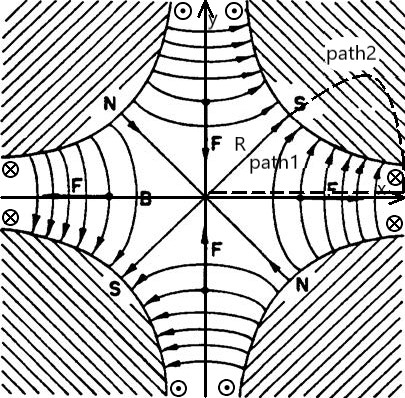
\includegraphics[scale=.7]{Homework_3Problem_1.jpg}
\caption{Problem 1} \label{Problem1}
\end{figure}
\end{sol}

\begin{problem}{2}
Find the potential of a uniformly charged ring with radius $R$ and line charge density $\tau$. Find the explicit function of the potential on the symmetry axis.
\end{problem}
\begin{sol}
We construct a rectangular coordinate system whose origin is the center of the charged ring, as shown in Figure \ref{Problem2}.The potential of the charged ring is
\begin{align*}
\phi(x,y,z)=&\frac{1}{4\pi\epsilon_0}\oint_{charged~ring}\frac{\tau dl}{r}\\
=&\frac{\tau}{4\pi\epsilon_0}\int_0^{2\pi}\frac{d\theta}{\sqrt{(x-R\cos\theta)^2+(y-R\sin\theta)^2+z^2}}
\end{align*}
The potential on the system axis ($z$ axis) is
\[
\phi(0,0,z)=\frac{\tau}{4\pi\epsilon_0}\int_0^{2\pi}\frac{d\theta}{\sqrt{R^2+R^2+z^2}}=\frac{\tau}{2\epsilon_0\sqrt{2R^2+z^2}}
\]
\begin{figure}[h]
\centering
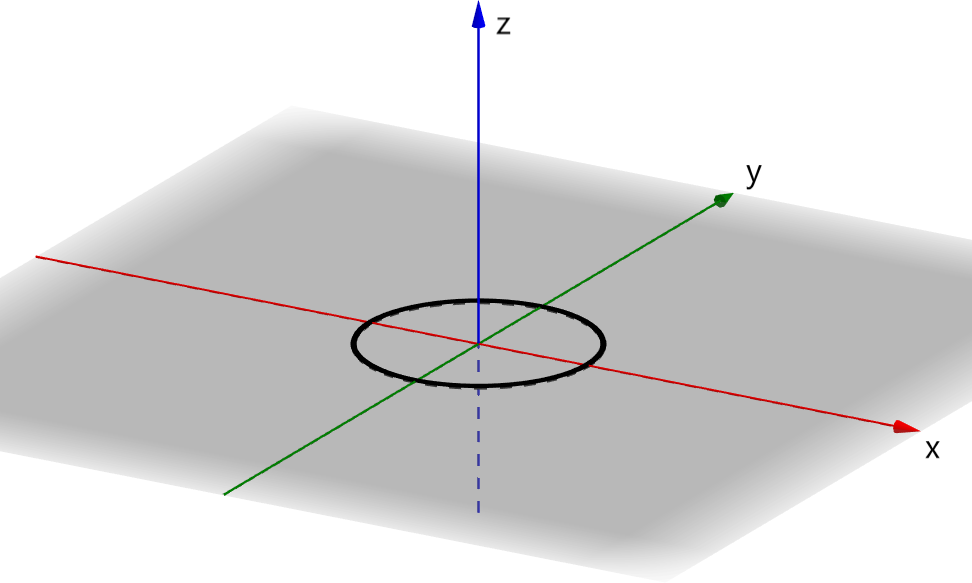
\includegraphics[scale=.3]{Homework_3Problem_2.png}
\caption{Problem 2} \label{Problem2}
\end{figure}
\end{sol}
\end{document}